\documentclass[12pt]{article}

\usepackage{hyperref}
\usepackage{caption}
\usepackage[margin=1.25in]{geometry}

\usepackage{graphicx}
\graphicspath{ {images/} }

\usepackage{minted}
\setminted[c++]{frame=single,linenos=true,autogobble=true,numbersep=4pt,tabsize=4}

\usepackage [english]{babel}
\usepackage [autostyle, english = american]{csquotes}
\MakeOuterQuote{"}


\begin{document}
\pagenumbering{gobble}
\begin{titlepage}
	\centering
	{\Huge C++ Retrofit Parralelization\par}
	\vspace{0.25in}
	{\Large Project 3\par}
	\vspace{2in}
	{Alex Harper\par}
	\newpage
\end{titlepage}
\pagenumbering{roman}

\tableofcontents
\newpage

\listoffigures
% \listoftables
\newpage
\setlength{\parindent}{4em}
\setlength{\parskip}{1em}

\pagenumbering{arabic}

\section{Introduction}

For the last project of the parralelization class, I decided to retrofit an older program of mine to multithread some of the algorithums.
The program already technically spawns several threads, but they are just basics to keep the GUI responsive while a single worker thread does work.
What I really want done is to multi-thread the algorithums that are run to make them faster on larger core count machines.

The focus that I had while doing the content of this paper was trying to interprit the current implementations, and finding the best places to try threading.
For this, OpenMP is fantasticly simple to use since many times you really are just wanting to do loops in parralel.
It also provides constructs to have a single line make certain instructions thread safe or add barriers.

\subsection{The Program}

Just a quick description of what the program is that I am working on.
The program is just a couple different algorithums to do stupid things to images.
There is no serious point to what they do besides they were interesting to work on and interesting to optimize.
They were never made with making them multi-threaded in mind.
This situation has topics of not only working with an older and not fully known code base, but also shows some common areas that get in the way of multi-threading.

\begin{figure}[htb]
	\centering
	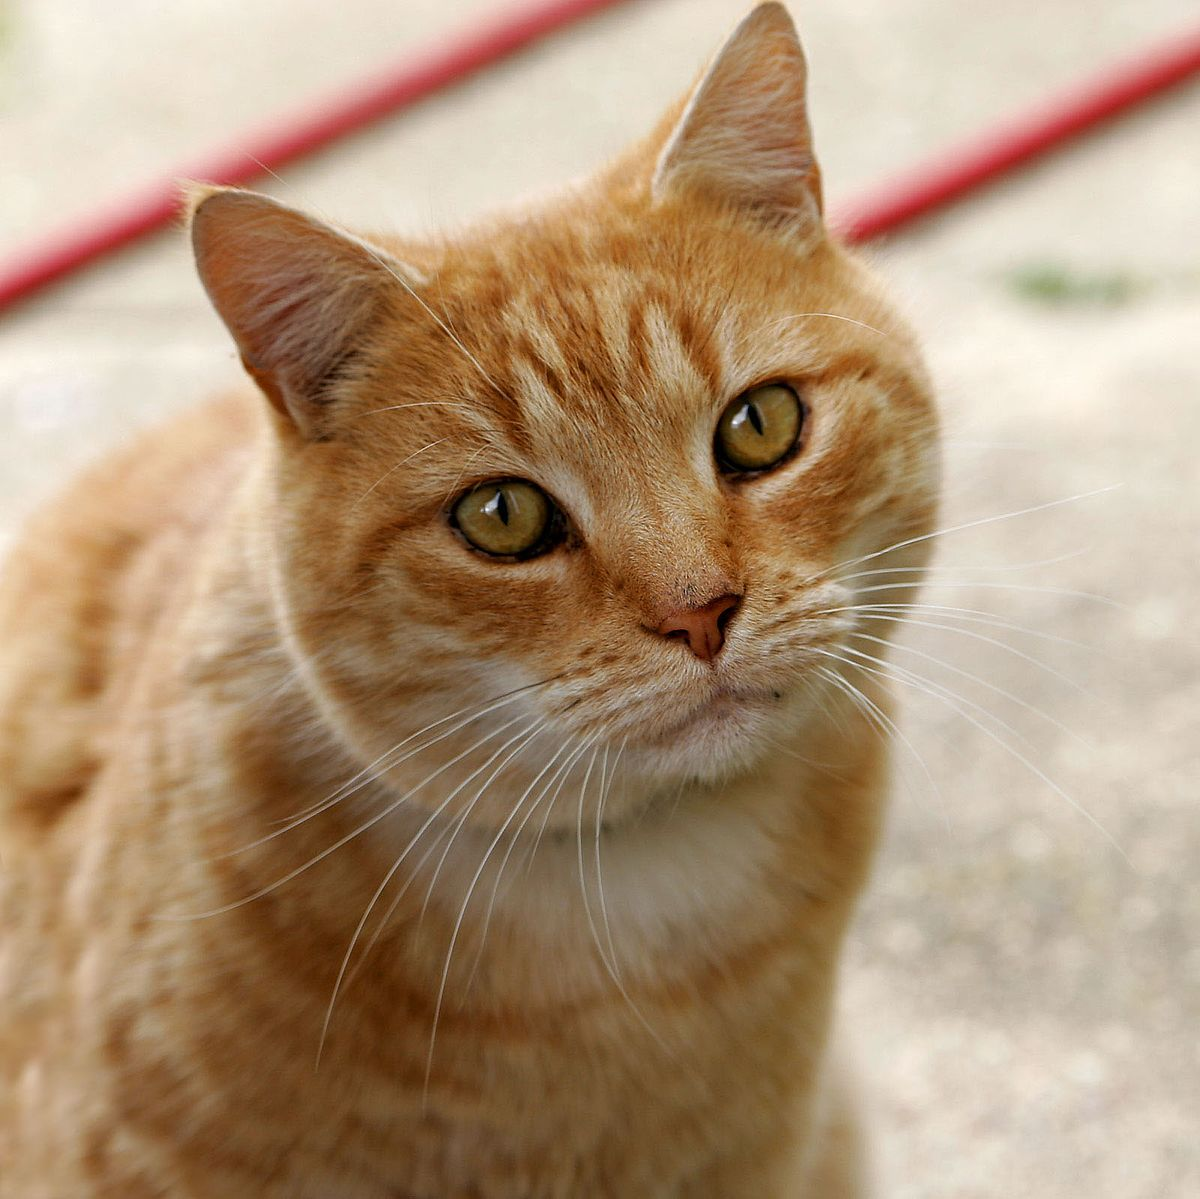
\includegraphics[width=0.3\textwidth]{example_source.jpg}
	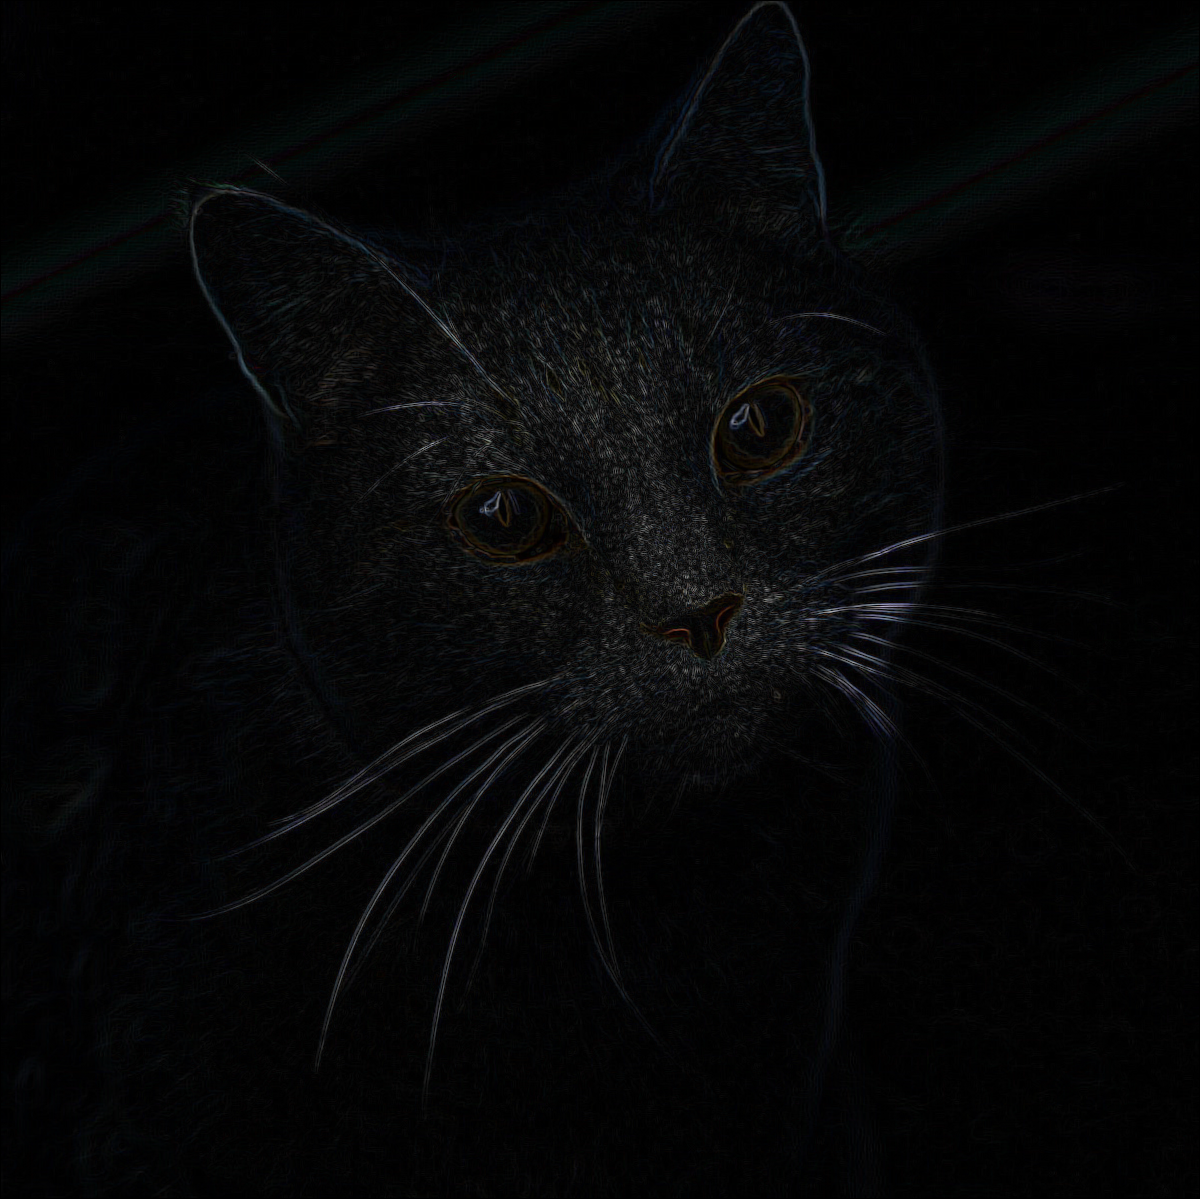
\includegraphics[width=0.3\textwidth]{example_edge.png}
	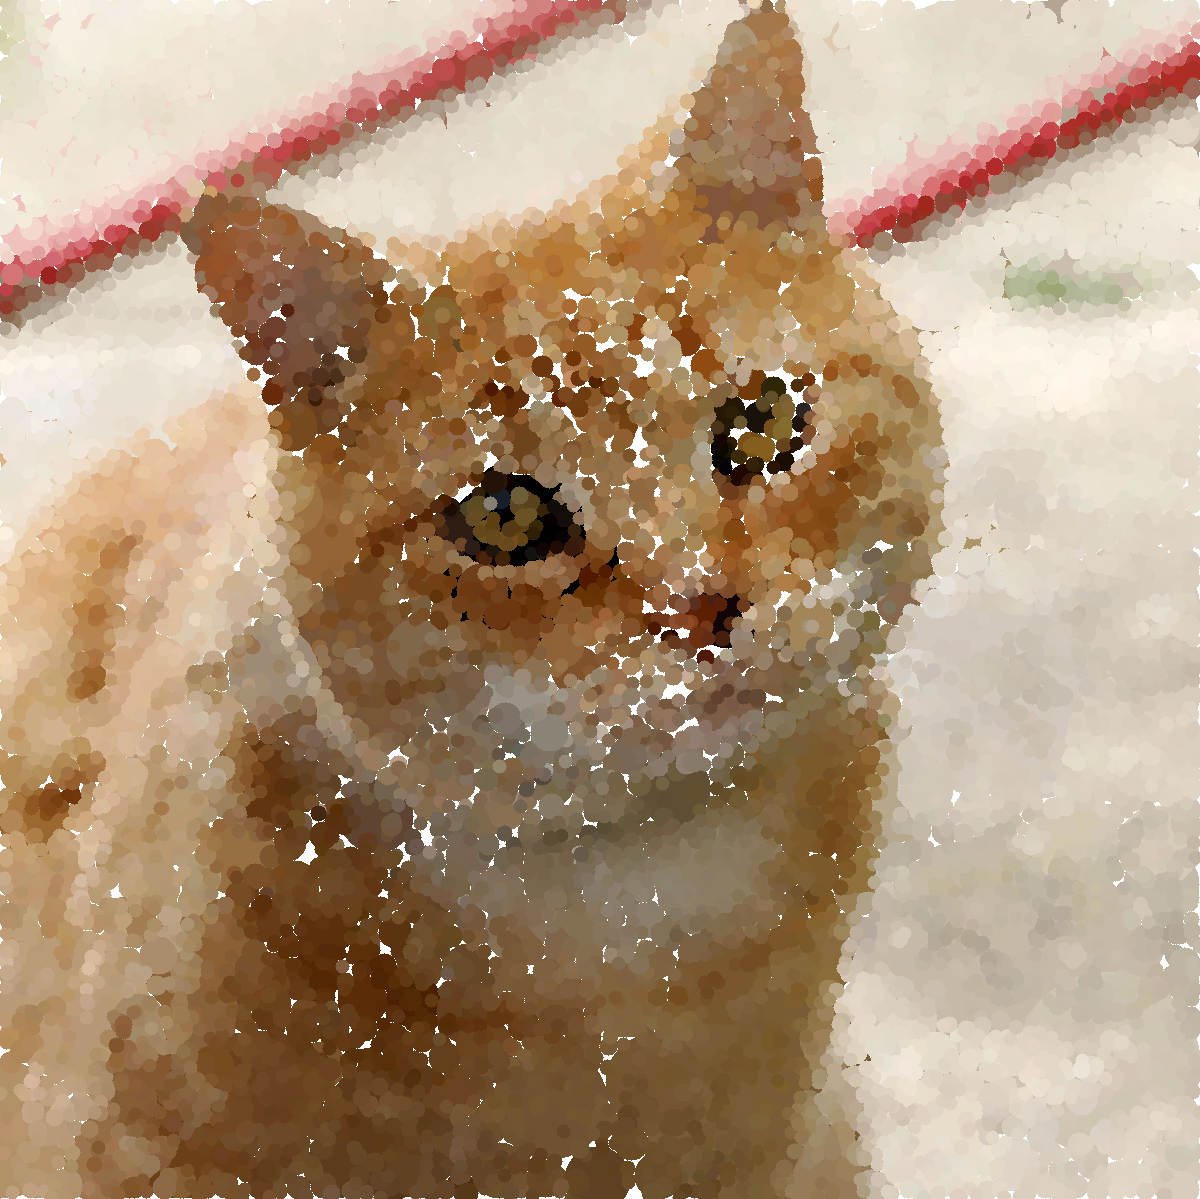
\includegraphics[width=0.3\textwidth]{example_circles.png}
	\caption{Example Images of the Two Main Algos}
\end{figure}

\newpage
\section{Edge Detector}

Starting with the simplest thing implemented, it should be a good point to practice analyzing the situation.
An edge detector is a fairly straight forward application of multiplying a matrix over an image.
The program starts with some hard coded default matrixes that give fair results and so I used these to test with.

The important thing to start with is to be at least passingly familiar with the system.
As such, I drew out a rough flowchart of what it does to apply the matricies to do the edge detection.
The image below is something I drew on my little whiteboard in my room.
The colored bubbles and lines are the loops, and so are likely method of adding threading.

\begin{figure}[htb]
	\centering
	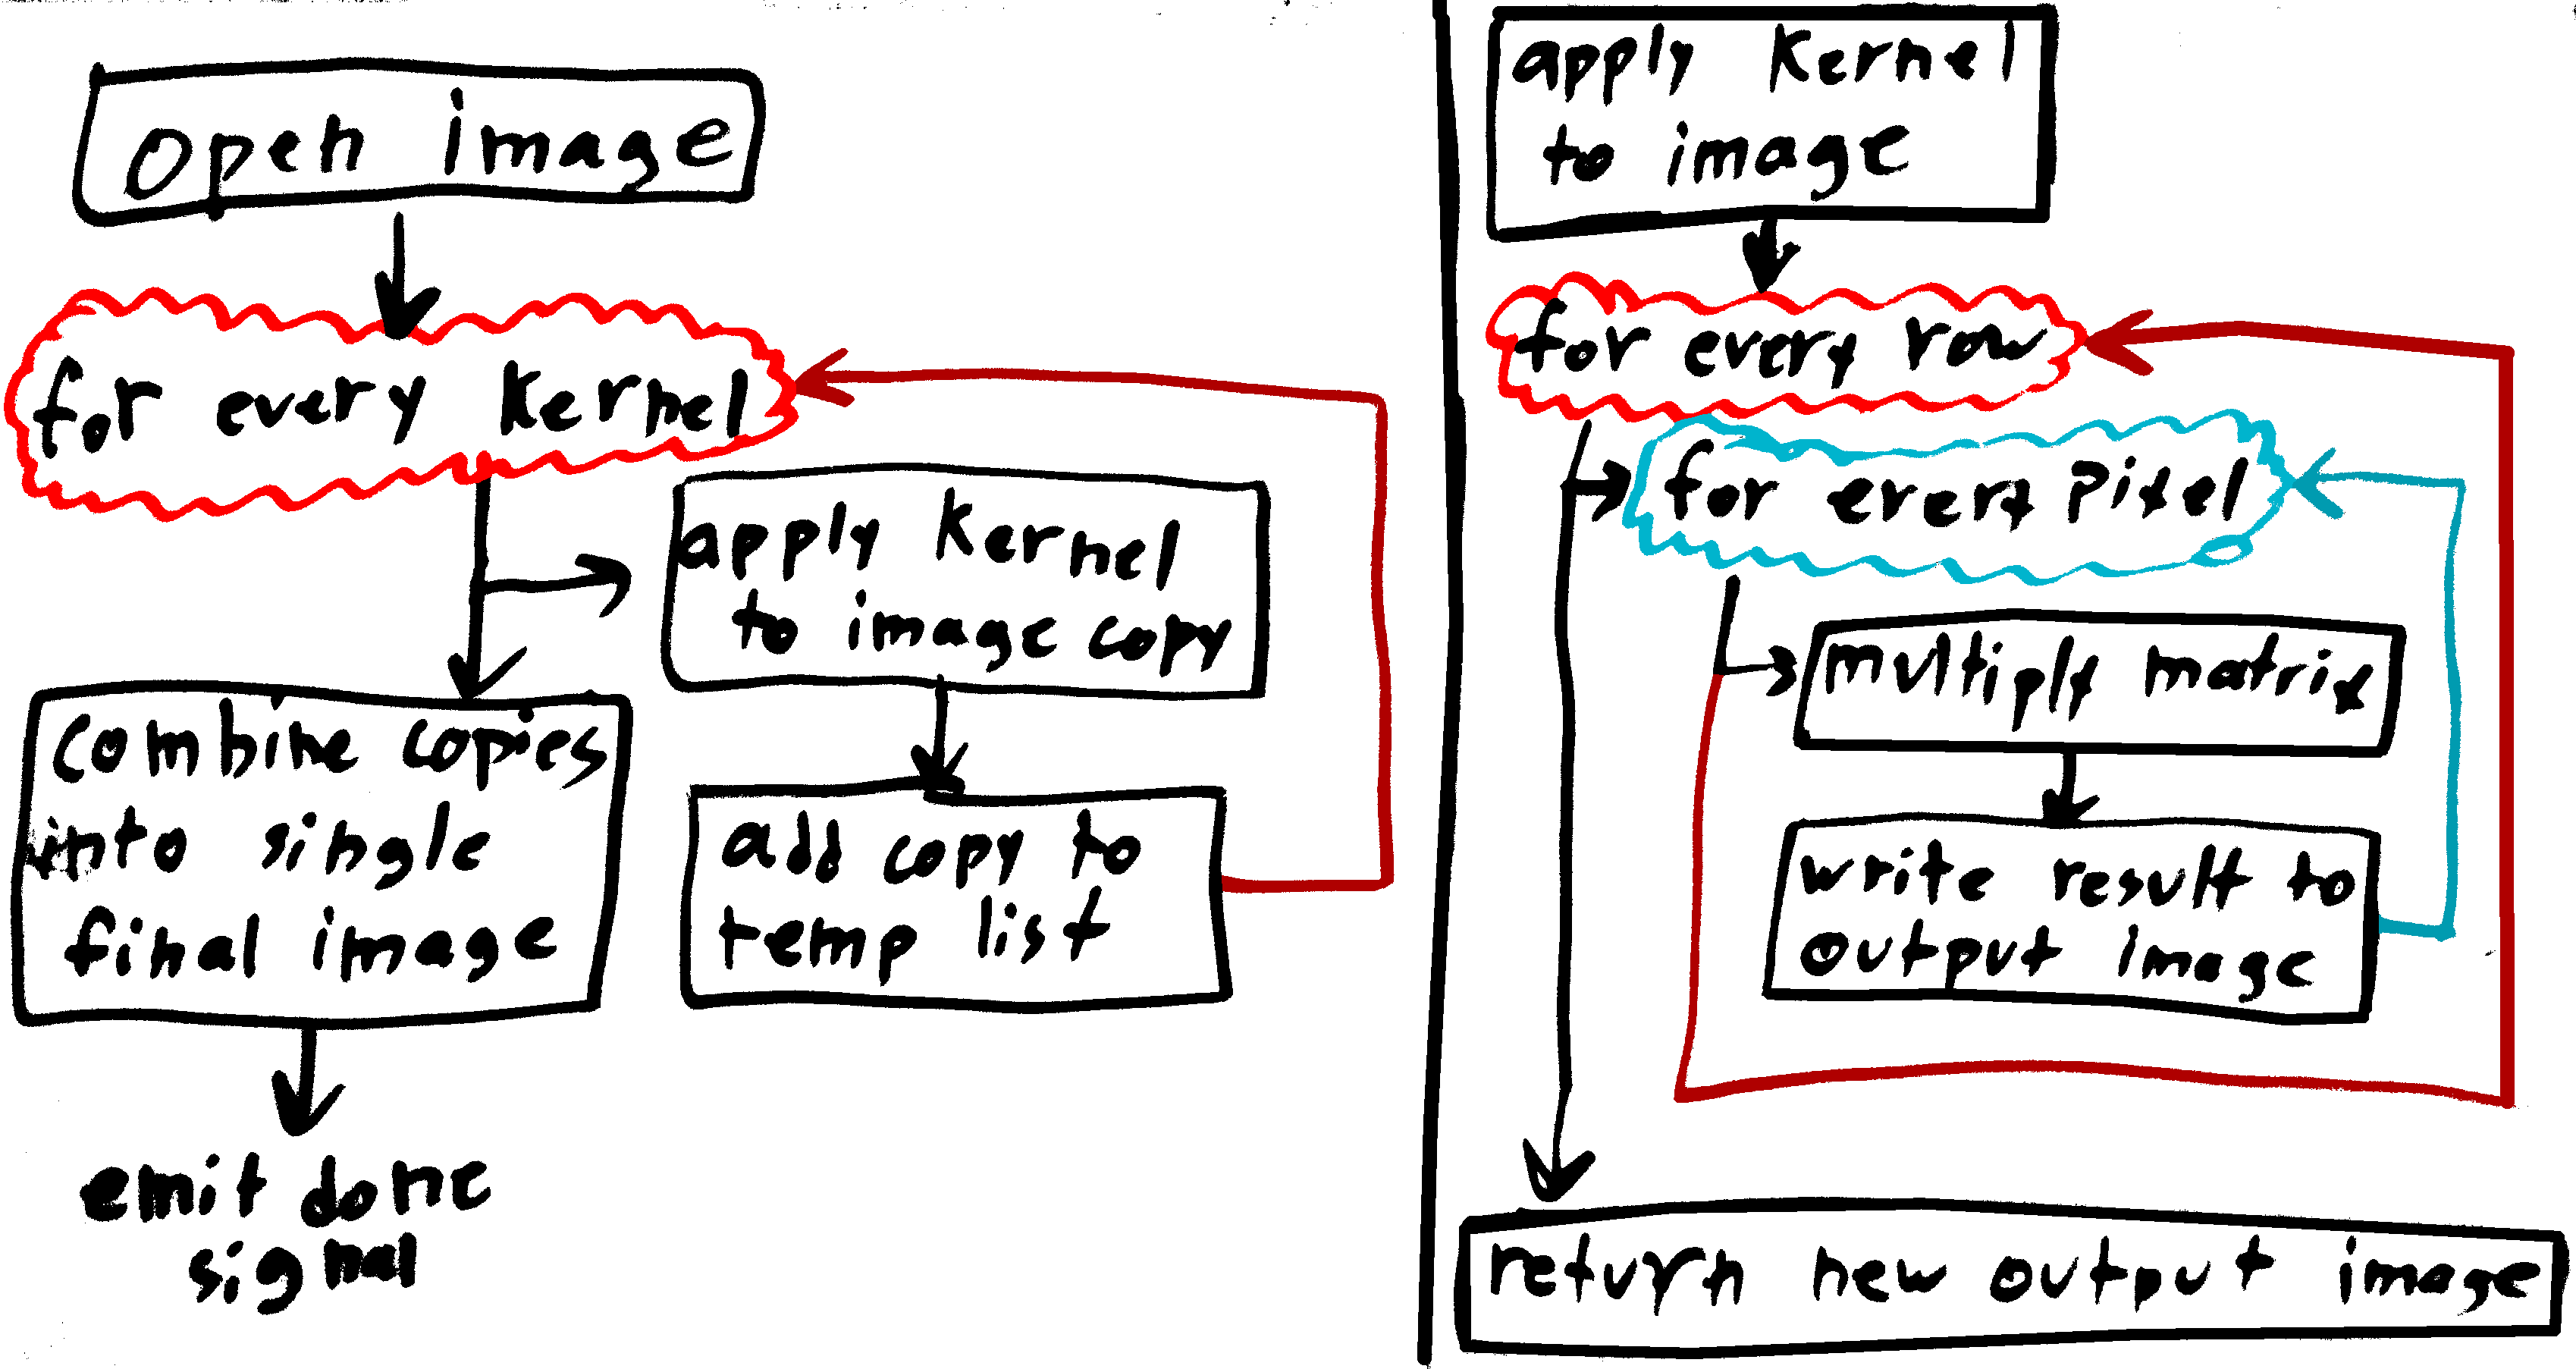
\includegraphics[width=0.7\textwidth]{edge_flowchart.png}
	\caption{Flowchart of how the edge detector works}
\end{figure}

Looking at the different loops, the loop on the left that does each kernel is the first loop in the algorithum.
I imediatly think that it is a bad choice for making parallel bacause it has so few items.
Each item is long lived which is good for making worker threads, but the number of items is low so in some cases the load could be uneven.

The right side shows the sub-step of applying a kernel to a copy of the image.
The two loops are for going through the pixels of the image and doing the multiplication at each.
There are a few ways to break it up:
\begin{itemize}
	\item Split number of rows evenly among threads
	\item Spawn threads and pass a single row at a time to each
	\item Have threads even split each row for each thread
	\item Have all the pixels evenly split between the threads
\end{itemize}

I believe that the first option will work the best, but as always, test everything.
The reason for my guess is that it is simple, and that you dont have things being passed around much.
Spawning the threads and giving them one line at a time will probably have more overhead of having to hand the job for every line.

Splitting each line to hand a different segment to each thread is likely going to suffer from small job sizes.
Each segment would only be a few kilobytes instead of whatever a full line size would be.
Splitting the bytes of the picture in total is a complicated thing, and so is also going to have overhead problems.
It woulde have to condense the two loops together and then give weird start and stop points in the middle of the loops.

\begin{figure}[htb]
	\centering
	\begin{tabular}{|c|c|c|}
		\hline
		Test Location & Average (ms) & Numbers \\ \hline \hline
		Baseline & 4930 & 4925,4936,4935,4923 \\ \hline
		Staticly Distributed Lines & 1400 & 1386,1409,1445,1362 \\ \hline
		Dynamically Distributed Lines & 1406 & 1368,1390,1497,1370 \\ \hline
		Split Pixels Per Line & 1556 & 1617,1463,1545,1600 \\ \hline
		Staticly Split Pixels & 1529 & 1522,1470,1571,1556 \\ \hline
		Dynamically Split Pixels & 1606 & 1559,1672,1612,1583 \\ \hline
	\end{tabular}
	\caption{Timings of multi threading the Edge Detector}
\end{figure}

After the tests, you can see that breaking the image up into different lines is the best way to do it speed wise.
I find it interesting how the different scheduals of breaking up the lines seems to not matter; the two timings are within margin of error.
Having the image broken up in a per pixel manner was consistently the slowest.

\subsection{Distributing Lines (OMP Schedules)}

The fastest way to break up the image between the threads was by throwing entire rows of pixels at each worker thread.
There is an important detail left out of what exactly is going on when we are doing that, something that OpenMP calls schedules.
This tells it how to break the loops down to hand to each thread.
The two main ways of giving out work are directly correlated to the schedules.

The first is the "static" schedule where before starting the threads, it divides the number of iterations by the number of threads being made.
The first chunk of iterations go to the first thread, the second chunk to the second thread, etc.
This is fine for loads that have each iteration take the same amount of time like here where we doing simple matrix math.
(ex 3 threads, 1 gets 0,1,2 , 2 gets 3,4,5 , 3 gets 6,7,8)

\begin{figure}[htb]
	\centering
	\begin{minted}{c++}
		#pragma omp parallel for schedule(static)
		for(line in picture)
			for(pixel in line)
				magic_matrix_math();
	\end{minted}
	\vspace{-16pt}
	\caption{Splitting the Lines (Static)}
\end{figure}

The second is the "dynamic" schedule where it starts the threads and then gives each thread a single iteration.
Every time a thread finishes its work, it asks for a new iteration to be given to it.
This is better for tasks where each iteration can take different amounts of time; a thread might get lucky and be handed a bunch of easy tasks while another thread is still churning away on its first.
(ex 3 threads, 1 gets 0,4 , 2 gets 1,3,5,8 , 3 gets 2,6,7)

\begin{figure}[htb]
	\centering
	\begin{minted}{c++}
		#pragma omp parallel for schedule(dynamic)
		for(line in picture)
			for(pixel in line)
				magic_matrix_math();
	\end{minted}
	\vspace{-16pt}
	\caption{Splitting the Lines (Static)}
\end{figure}

\subsection{Distributing Pixels (OMP Collapse)}

The least fast way of threading was splitting up the full bytes of the picture.
Instead of having fulls rows assigned to each thread, the image was split up along all the pixels.
To get this to happen, there is a single argument to add to the parralel directive.
This is interesting for OpenMP even though I see limited usefulness for it.

\begin{figure}[htb]
	\centering
	\begin{minted}{c++}
		#pragma omp parallel for collapse(2)
		for(line in picture)
			for(pixel in line)
				magic_matrix_math();
	\end{minted}
	\vspace{-16pt}
	\caption{Splitting Across Multiple Loops}
\end{figure}

This code snippet has the "collapse" directive which tells OpenMP to split nested loops.
It now will split the values for the two loops into independent chunks, like saying (row 10,column 20) to be passed to each thread.
This makes each pixel a potential target for a worker thread to work on while having no regards to what row they are on.
The only requirment is that the inner loops are not dependent on the value of outer loops.

\subsection{Combining Images}

And so after looking and thinking about what loops to make parallel and making the kernel math faster, there was one other place.
The step of "combine the copies" is where it loops through all the pixels again and adds everything together into a final image.
There was not much thought to this as it is just applying what is discussed above to a slightly different loop.

\begin{figure}[htb]
	\centering
	\begin{tabular}{|c|c|}
		\hline
		Test Location & Time (ms) \\ \hline \hline
		Baseline & 2343 \\ \hline
		Distributed Lines & 765 \\ \hline
	\end{tabular}
	\caption{Timings of multi threading the Edge Detector}
\end{figure}

\newpage
\section{Random Circles}

Now we can focus on the more complicated approximator the program has; drawing circles on a blank picture similar to \href{https://en.wikipedia.org/wiki/Pointillism}{pointillism}.
This is a more convoluted algorithim where it randomly places a circle, and then tries to move it around or make it larger and smaller.
It decides what changes are best by getting an average color delta between the current approximation and what the new circle will instead have.

%Methods to parallelize
%each thread makes a circle and optimizes, then they all wait on each other and then draw
%each thread takes an area of the picture to optimize a sub-set of circles for

Like before, I started by drawing out the rough flowchart of how it works.
There is only a single main loop that does all the work, with the complicated bits hidden in the looping steps.
So it seems obvious to have each thread work on its own circle.

\begin{figure}[htb]
	\centering
	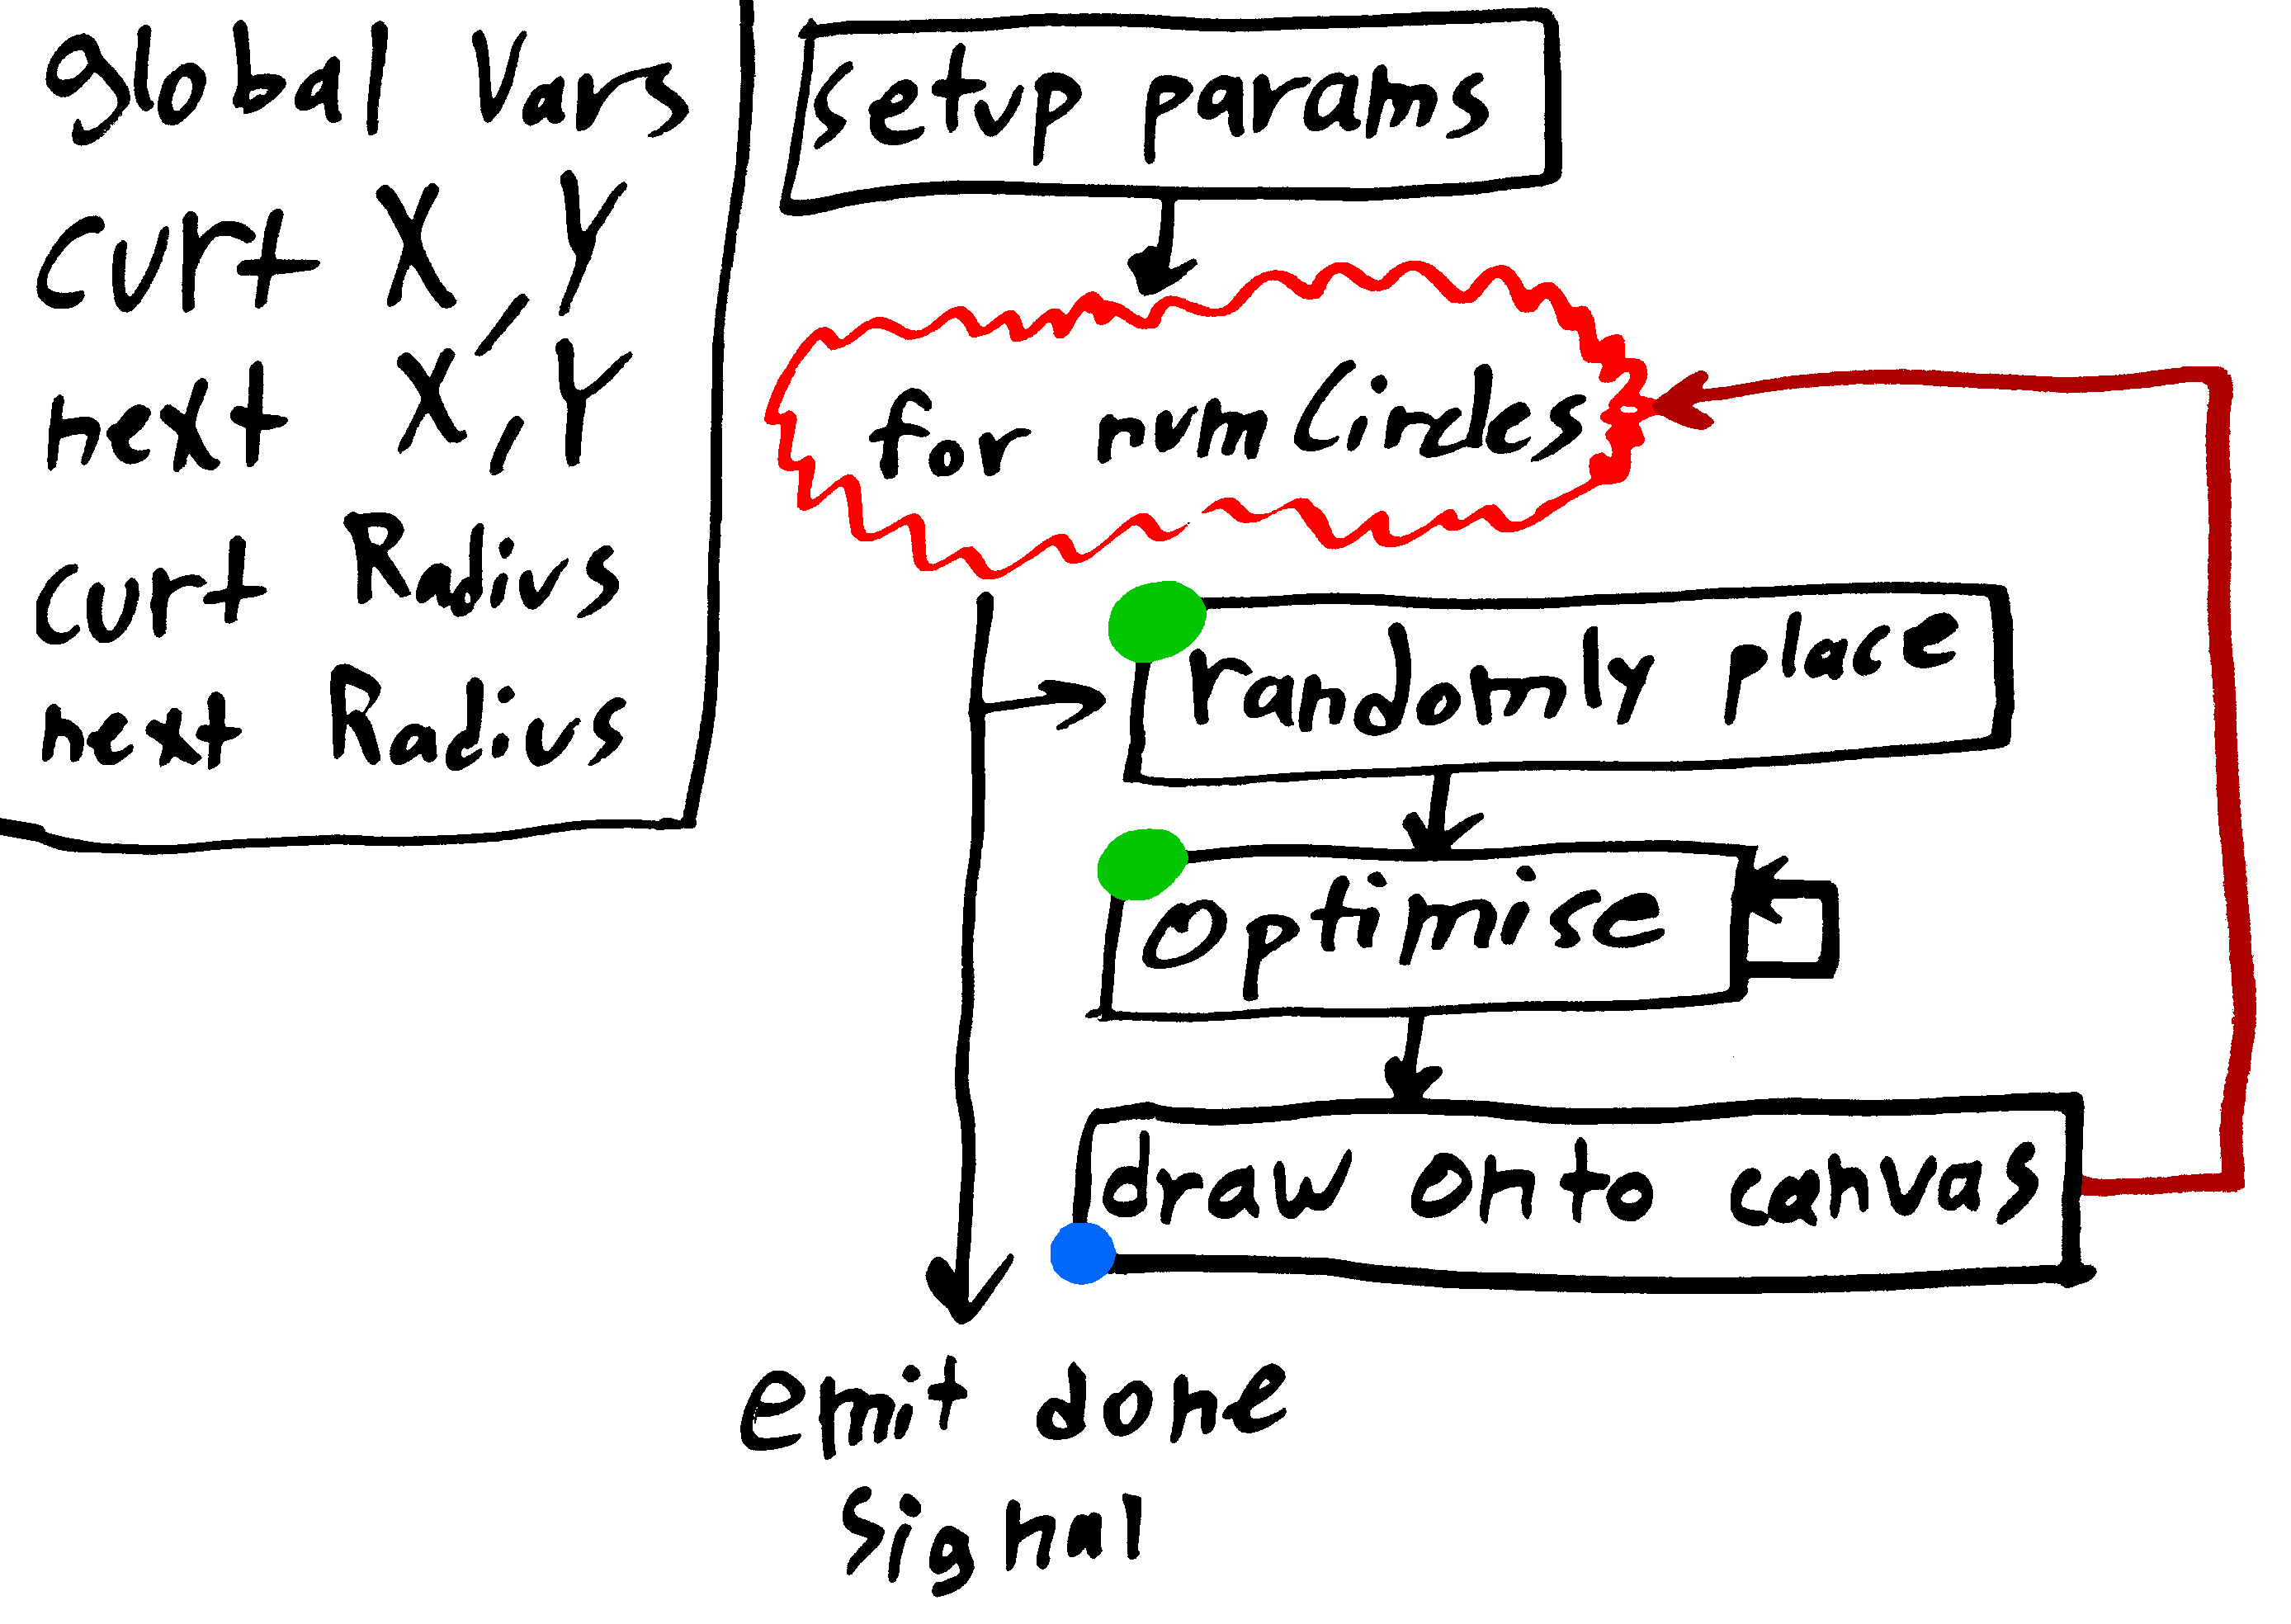
\includegraphics[width=0.6\textwidth]{circle_flowchart.png}
	\caption{Flowchart of how the Cirlce Approximator works}
\end{figure}

As you can see on the left side, there are some global variables that are used in different methods.
The steps that have the green dot on them use and change these global variables.
This is a problem, as they will be shared between threads and each thread will trash the data the others are trying to use.
Problems such as this are going to be common for code that was never intended to be threaded, and will always require a refactor to fix it.

There is also the last step of drawing the circles to the picture.
Due to the nature of the algorithum, this must stay globaly shared between the threads since this is where all the drawn circles are collected.
Luckily OpenMP has some ways to deal with that.

\subsection{Refactor Global Variables}

Looking at the various variables, it seems they are for simply describing the current circle being considered.
Since they are all related to a single task, it is probably best to wrap them up together.

\begin{figure}[htb]
	\centering
	\begin{tabular}{|p{0.425\textwidth}|p{0.475\textwidth}|}
	\hline
	Before & After \\ \hline \hline
	\begin{minted}[frame=none,linenos=false,autogobble=true,numbersep=0pt]{c++}
		int curtX, curtY;
		int nextX, nextY;
		int curtRadius, nextRadius;
	\end{minted}
	&
	\begin{minted}[frame=none,linenos=false,autogobble=true,numbersep=0pt]{c++}
		struct Circle{
			int curtX, curtY;
			int nextX, nextY;
			int curtRadius, nextRadius;
		}
	\end{minted}
	\\ \hline
	\begin{minted}[frame=none,linenos=false,autogobble=true,numbersep=0pt]{c++}
		void modifyGlobalsForATask();
	\end{minted}
	&
	\begin{minted}[frame=none,linenos=false,autogobble=true,numbersep=0pt]{c++}
		void modifyLocalStruct
				(struct Circle * circle);
	\end{minted}
	\\ \hline
	\end{tabular}
	\caption{Factoring Out Global Variables}
\end{figure}

This way has every iteration of the loop will have its own independant struct and will pass it to the various methods to modify it.
A simple fix in principle, but takes time to change everything for the different syntax.
With how deeply embedded the globals were used, it took a bit of time to work it all out.

\newpage
\subsection{Global Final Canvas}

\begin{figure}[htb]
	\centering
	\begin{minted}{c++}
		#pragma omp parallel for schedule(dynamic)
		for(int circle : circles_wanted){
			struct Circle circle;
			randomlyPlace(&circle);
			optimize(&circle);
			draw(circle);
		}
	\end{minted}
	\caption{Baseline Parallel Code}
\end{figure}

This is another interesting thing to work on.
The canvas that all the circles are drawn onto has to be global to collect all the various made dots.
But the canvas is not a simple write only collection point, but is used when optimizing the circles.
The circles have to be a better approximation over an area that what the current canvas holds otherwise what is the use of the circle.

As such, we can't have the canvas change when one thread is done optimizing if another thread is still busy using it.
To keep this from happening, OpenMP has things called "barriers".
A barrier makes a thread pause when it encounters it, and it waits until all the other threads have caught up to it.
If we put a barrier before the draw command, we can be certain that all the threads have finished with their tasks and so is safe to modify the drawing.

\begin{figure}[htb]
	\centering
	\begin{minted}{c++}
		#pragma omp parallel for schedule(dynamic)
		for(int circle : circles_wanted){
			struct Circle circle;
			randomlyPlace(&circle);
			optimize(&circle);
			#pragma omp barrier
			draw(circle);
		}
	\end{minted}
	\caption{Barrier Before Drawing}
\end{figure}

With all the threads pausing before drawing, we can see another problem.
Since they are all trying to change the same resource, we can never be certain the threads are not writing over top of each other.
If two threads have circles that will overlap, what will it do?
There will be some odd looking cases of circles half drawn over each other.
(assuming the threads draw on the same line at the same time, and how the cache flushes the pixels back, and etc etc etc)

Even though my gut tells me that it is a tiny problem, I still feel that it is best to keep threads from stepping on each other.
This means we need to make the drawing command single threaded and only write one thing at a time.
OpenMP lets us specify this by simply saying a certain line or block is critical.

\begin{figure}[htb]
	\centering
	\begin{minted}{c++}
		#pragma omp parallel for schedule(dynamic)
		for(int circle : circles_wanted){
			struct Circle circle;
			randomlyPlace(&circle);
			optimize(&circle);
			#pragma omp barrier
			#pragma omp critical
			draw(circle);
		}
	\end{minted}
	\caption{Drawing is a Critical Command}
\end{figure}

And now that we are drawing one at a time, there is another problem.
Lets say there are 2 threads; thread 1 finishes drawing and will go back to the top of the loop while thread 2 starts drawing.
That will be the same problem that we started with, where 1 is trying to use the canvas while 2 is drawing to it still.
That is another easy fix of just have all the threads wait after they are done drawing.

\begin{figure}[htb]
	\centering
	\begin{minted}{c++}
		#pragma omp parallel for schedule(dynamic)
		for(int circle : circles_wanted){
			struct Circle circle;
			randomlyPlace(&circle);
			optimize(&circle);
			#pragma omp barrier
			#pragma omp critical
			draw(circle);
			#pragma omp barrier
		}
	\end{minted}
	\caption{Barrier After Drawing}
\end{figure}

And there you go, multithreaded circle optimization but single threaded drawing.

\subsection{But Wait, It Doesn't Work}

Ah, there is always a wrench in the plan.
While theoretically the above code would work just fine, the snag is with OpenMP.
The "barrier" commands do not work inside a loop construct and just throw compiler errors.
This means that we must do it in a more round-about way.
(though honestly compared to what I was expecting to have to do, is not much trouble at all)

The way this will happen is that we will not use the simple built-in for-loop thing that OpenMP has.
We will instead have it spawn the threads, divide how many things each loop needs to do, and then use a loop.
Then the same sequence of events as discussed above can happen unmodified.

\begin{figure}[htb]
	\centering
	\begin{minted}{c++}
		#pragma omp parallel
		{
			int num_threads;
			int circlesPerThread;
			#pragma omp critical
			{
				num_threads = omp_get_num_threads();
				circlesPerThread = numCircles / num_threads;
			}

			for(int circle; circle<circlesPerThread; circle++){
				struct Circle circle;
				randomlyPlace(&circle);
				optimize(&circle);
				#pragma omp barrier
				#pragma omp critical
				draw(circle);
				#pragma omp barrier
			}
		}
	\end{minted}
	\caption{Not Using OpenMP "for" Construct}
\end{figure}

Lets break down what that code snippet is doing.

The first pragma is telling OpenMP to spawn the threads and start running the block in parallel.
This means that starting with creating the private variable "num\_threads" is already running is parallel.
Since it is simply code running in parallel, you have to handle it closer to the way pthreads work.

The second pragma is a "critical" section where it only allows a single thread to run at a time.
This is because (ironicly) the omp\_*() functions are not thread-safe.
We decide on some basic parameters for what each thread will operate on, namely how many circles go to each thread.

The third part is the for loop.
The contents is exatly the same as previously discussed, except that the barriers now work!
This makes it almost an exact feature parity as the built-in for-loop construct.

\subsection{Embelishing}

After getting the basics of the thing working, there is always more that can be done.
For example, the code above does not show it giving progress updates back to the GUI thread.
That code is in the final program, but there is something special.
Since it is supposed to just be a rough progress report to the user, it is silly to have every thread throw back the same image to the GUI.
So using OpenMP, we can ask it to only have the master thread run a slice of code while the other threads will jump over it.

\begin{figure}[htb]
	\centering
	\begin{minted}{c++}
		#pragma omp master
		{ // emit details of progress
			double percentage = (circle_num+1)/(double)numCircles*100;
			emit progressMade(currentApproximation,percentage);
			QCoreApplication::processEvents();
		}
	\end{minted}
	\caption{Master Thread Only Runs This Code}
\end{figure}

There is also a thing in the program that I like to have; a stop button.
As the code presented sits, there is no way to have the threads stop early.
I have things piped up already to have a global bool get set to false when the stop button is pressed.
The code below is my first attempt at getting the threads to stop.

\begin{figure}[htb]
	\centering
	\begin{minted}{c++}
		bool keepGoing;
		#pragma omp parallel
		{
			while(circle_num<circlesPerThread && keepGoing){
				#pragma omp barrier
				draw(circle);
				#pragma omp barrier
			}
		}
	\end{minted}
	\caption{Incorrect Stop Flag}
\end{figure}

The problem with this is the boolean "keepGoing" is non-atomic.
When the value gets changed externally by the GUI thread, the time it takes to propgate the value into the running threads is indeterminate.
That means that some thread might exit while another thread gets stuck on the barrier before drawing the circle.
Since a thread got stuck, that means we got to a bad program state.
The way to fix this is to force the value to be consistent between threads before using it.
C++11 standard introduced a fantastic wrapper, std::atomic, that handles it transparently.

\begin{figure}[htb]
	\centering
	\begin{minted}{c++}
		std::atomic<bool> keepGoing;
		#pragma omp parallel
		{
			while(circle_num<circlesPerThread){
				#pragma omp barrier
				draw(circle);
				#pragma omp barrier
				if(!keepGoing) break;
			}
		}
	\end{minted}
	\caption{Correct Stop Flag}
\end{figure}

\end{document}
